\documentclass{beamer}

\usepackage[sfdefault]{cabin}
\usepackage[utf8]{inputenc}
\usepackage[T1]{fontenc}
\usepackage[french]{babel}
\usepackage{xcolor}
\usepackage{caption}
\usepackage{graphicx}
%Police
%\usepackage[sfdefault]{roboto}
\usepackage[sfdefault]{FiraSans}

\definecolor{modernmarron}{RGB}{88, 41, 0} 

\usetheme{Madrid}

\usecolortheme[named=modernmarron]{structure}

\setbeamertemplate{caption}{\insertcaption} % Utiliser le format de légende par défaut de Beamer

\title{Soutenance projets statistique en grande dimension }
\author{Ivanhoé Botcazou}
\date{22 janvier 2024}

\renewcommand{\thesection}{\Roman{section}}\renewcommand{\thesubsection}{\arabic{subsection} }\renewcommand{\thesubsubsection}{\alph{subsubsection} }

\newcommand{\C}{\mathbb{C}}\newcommand{\R}{\mathbb{R}}\newcommand{\Q}{\mathbb{Q}}\newcommand{\Z}{\mathbb{Z}}\newcommand{\N}{\mathbb{N}}\newcommand{\V}{\overrightarrow}\newcommand{\Cs}{\mathscr{C}}\newcommand{\Ps}{\mathscr{P}}\newcommand{\Rs}{\mathscr{R}}\newcommand{\Gs}{\mathscr{G}}\newcommand{\Ds}{\mathscr{D}}\newcommand{\happy}{\huge\smiley}\newcommand{\sad}{\huge\frownie}\newcommand{\alors}{\Large\Rightarrow}\newcommand{\equi}{\Leftrightarrow}
\newcommand{\disp}{\displaystyle}\newcommand{\Pro}{\mathbb{P}}


\newtheorem{thm}{Théorème}
\newtheorem{rmq}{Remarque}
\newtheorem{prop}{Propriété}
\newtheorem{cor}{Corollaire}
\newtheorem{lem}{Lemme}
\newtheorem{prop-def}{Propriété-définition}
\newtheorem{con}{Conclusion}

\theoremstyle{definition}

\newtheorem{defi}{Définition}
\newtheorem{intro}{Initialisation}
\newtheorem{boucle}{Boucle principale}
\newtheorem{ex}{Exemple}
\newtheorem*{rap}{Rappel}
\newtheorem{cex}{Contre-exemple}
\newtheorem{exer}{Exercice} % \large {\fontfamily{ptm}\selectfont EXERCICE}
\newtheorem{nota}{Notation}
\newtheorem{ax}{Axiome}
\newtheorem{appl}{Application}
\newtheorem{csq}{Conséquence}
\def\di{\displaystyle}



\begin{document}
\begin{frame}[plain]
    \maketitle
\end{frame}


\begin{frame}
\frametitle{Introduction}
\hfill\\[-0.75cm]
\begin{figure}
	\centering
	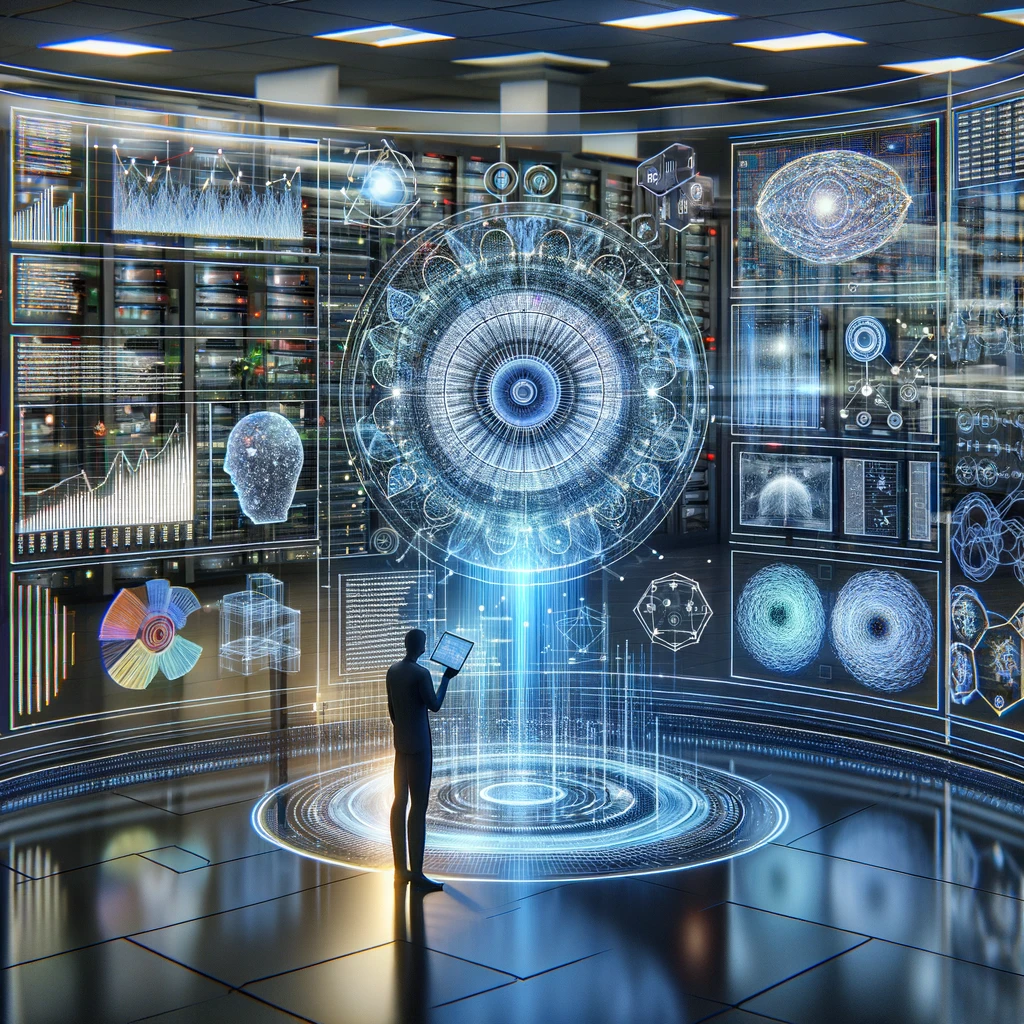
\includegraphics[width=0.55\linewidth]{1.png}\\[0.25cm]
	\raggedright
	\textcolor{modernmarron}{\textbf{Problématique :}} Comment utiliser l’apprentissage automatique pour résoudre des tâches complexes sur des grands jeux de données ?  
	
\end{figure}
\end{frame}

\begin{frame}
	\tableofcontents
\end{frame}

\section{La base de données MNIST}
\begin{frame}
	\frametitle{KNN avec la base de données MNIST}
		\begin{minipage}[c]{1\linewidth}
		\begin{minipage}[c]{0.5\linewidth}\centering\begin{figure}
				\centering
				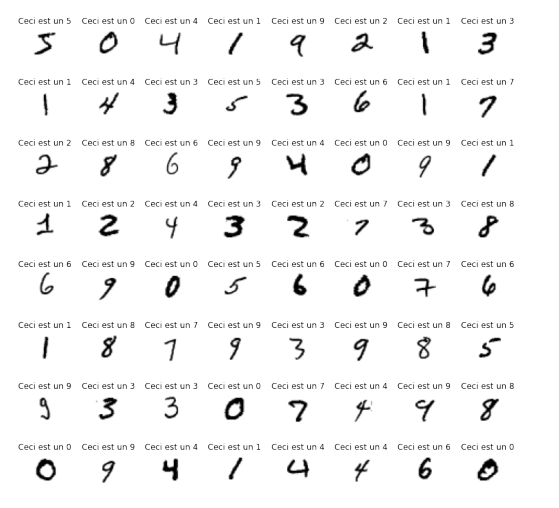
\includegraphics[scale=0.28]{MNIST.png}
				\caption*{Visualisation des données}
				
		\end{figure}\end{minipage}\hfill 
		\begin{minipage}[c]{0.48\linewidth}\centering\begin{figure}
				\begin{center}
					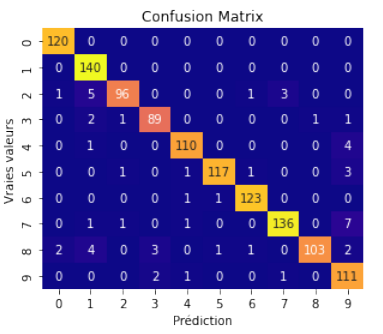
\includegraphics[width=1\linewidth]{3.png}			
					\caption*{Matrice de confusion KNN\_10}
				\end{center}
				
		\end{figure}\end{minipage}
	\end{minipage}	
\end{frame}

\begin{frame}
	\frametitle{Mauvaises prédictions du modèle}
	\begin{figure}
		\centering
		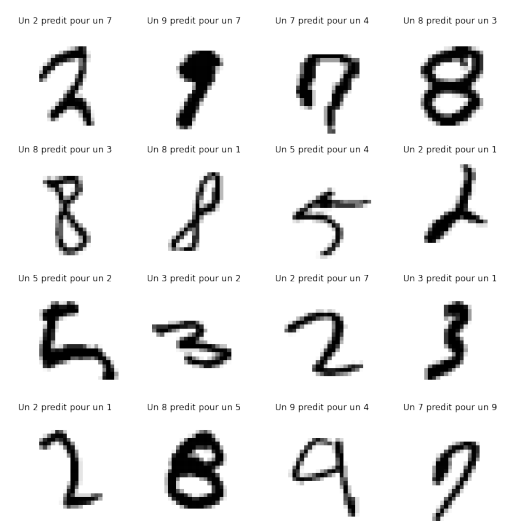
\includegraphics[width=0.55\linewidth]{4.png}\\[0.25cm] 
		
	\end{figure}
\end{frame}

\section{Classification de cancers}

\begin{frame}
	\frametitle{Classification des cancers avec des arbres de décisions}
	\hfill\\[-0.7cm]
	\begin{figure}
		\centering
		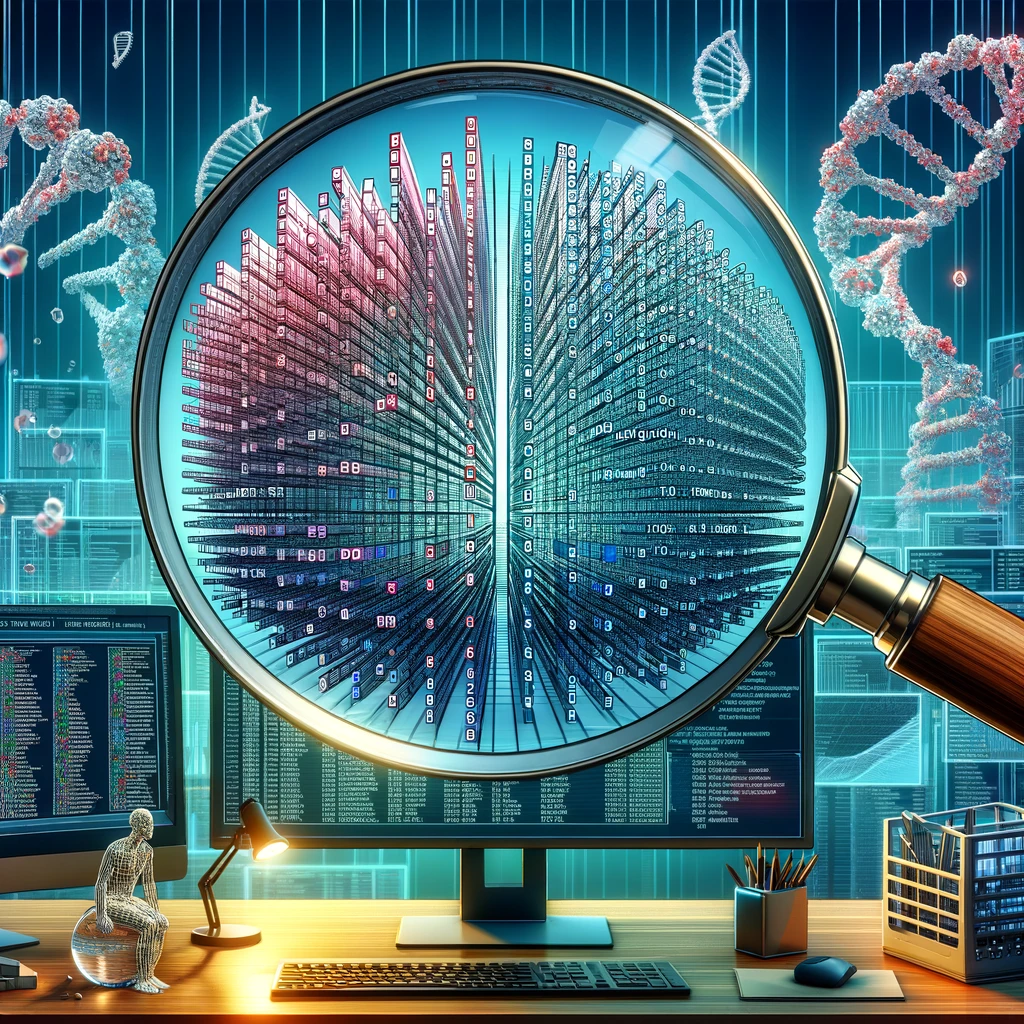
\includegraphics[width=0.4\linewidth]{cancers.png}
		
		\raggedright
		\hfill\\[-0.6cm]
		\begin{rmq}
			Classification de cancer en fonction de ses caractéristiques génétiques, couvrant un grand nombre de gènes. La difficulté réside dans le fait qu’il y a peu d’individus (143) pour un nombre très élevé de colonnes (16 063).
		\end{rmq}
		
		
	\end{figure}
\end{frame}

\begin{frame}
	\begin{minipage}[t]{1\linewidth}
		\begin{minipage}[t]{0.49\linewidth}\centering\begin{figure}
				\centering
				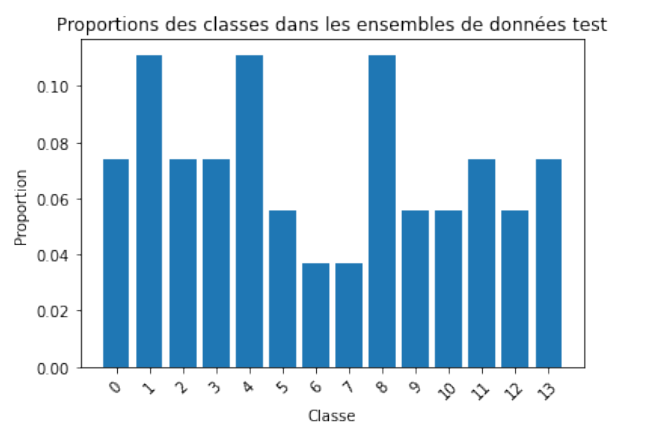
\includegraphics[width=1\linewidth]{8.png}
				%\caption*{Classes déséquilibrées }
				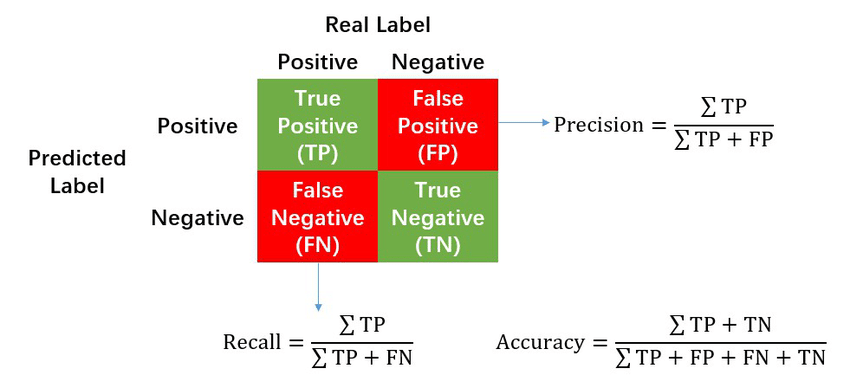
\includegraphics[width=1\linewidth]{7.png}
				%\caption*{Métriques de validation}
		\end{figure}\end{minipage}\hfill 
		\begin{minipage}[t]{0.49\linewidth}\centering\begin{figure}
				\begin{center}
					\centering
					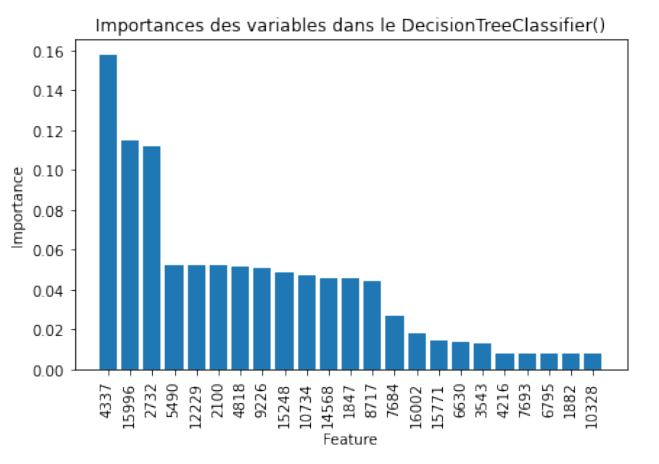
\includegraphics[width=1\linewidth]{10.png}
					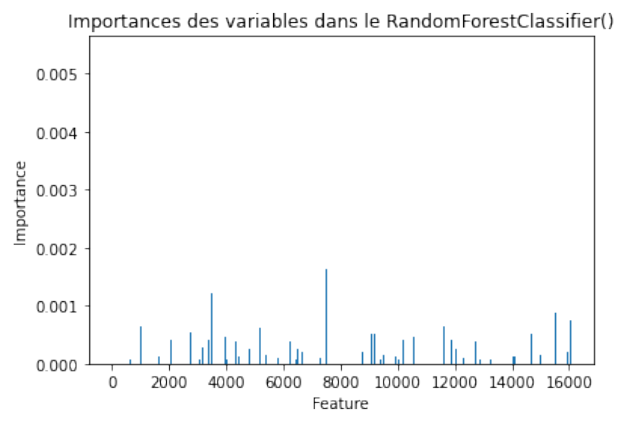
\includegraphics[width=1\linewidth]{11.png}
				\end{center}
				
		\end{figure}\end{minipage}
	\end{minipage}	
\end{frame}

\section{Algorithmes de Boosting avec des arbres}
\begin{frame}
	\frametitle{Gradient Boosting pour un problème de régression}
	
		\begin{minipage}[t]{1\linewidth}
		\begin{minipage}[t]{0.5\linewidth}\centering\begin{figure}
			\raggedright	
			Le but de cet algorithme est de construire un estimateur $F\in Lin\mathcal{(F)}$, où $\mathcal{F}$ est l'ensemble des arbres de décision de profondeur $p$ et $Lin\mathcal{(F)}$ est l'ensemble des combinaisons linéaires d'éléments de $\mathcal{F}$.
			
			Considérons la fonction de coût $$\Psi(z, y)= \dfrac{(z-y)^2}{2} $$
			
			L'objectif est de trouver $F^*$ qui minimise $C(F) = E[\Psi(F(X),Y)] $
			
			
		
			
				
		\end{figure}\end{minipage}\hfill 
		\begin{minipage}[t]{0.48\linewidth}\centering\begin{figure}
				\begin{center}
					\centering
					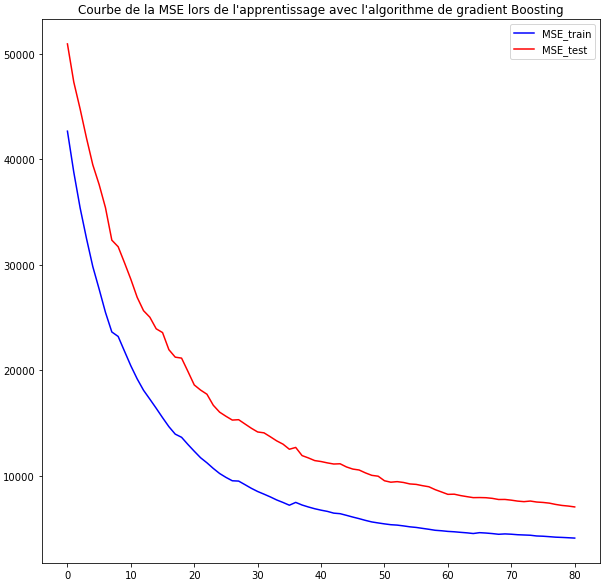
\includegraphics[width=1\linewidth]{reg_boost.png}
					
				\end{center}
				
		\end{figure}\end{minipage}
	\end{minipage}
	
\end{frame}

\begin{frame}
	\frametitle{Adaboost pour un problème de classification binaire }
		\begin{minipage}[t]{1\linewidth}
		\begin{minipage}[t]{0.53\linewidth}\centering\begin{figure}
				\centering
				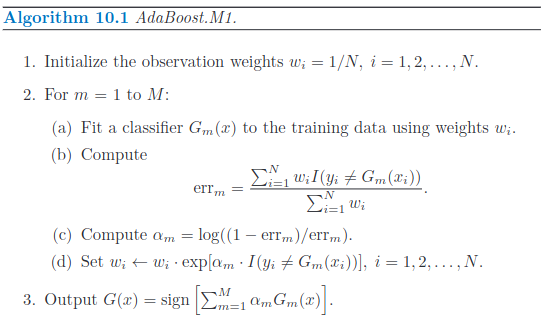
\includegraphics[width=1\linewidth]{adaboost0.png}
				Algorithme extrait du livre :\\ "The elements of statistical learning" 
		\end{figure}\end{minipage}\hfill 
		\begin{minipage}[t]{0.47\linewidth}\centering\begin{figure}
				\begin{center}
					\centering
					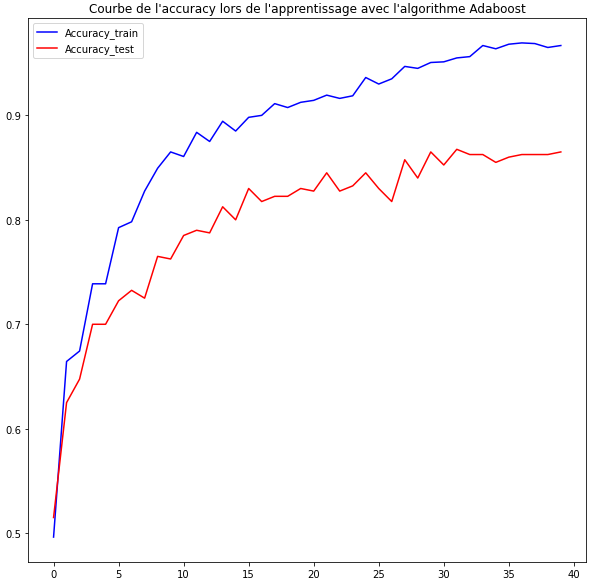
\includegraphics[width=1\linewidth]{adaboost1.png}
				\end{center}
				
		\end{figure}\end{minipage}
	\end{minipage}
	
\end{frame}

\begin{frame}
	\frametitle{Gradient Boosting pour un problème de classification multi-classe}
	
		\centering
	\begin{minipage}[c]{0.6\linewidth}\centering\begin{figure}
			
			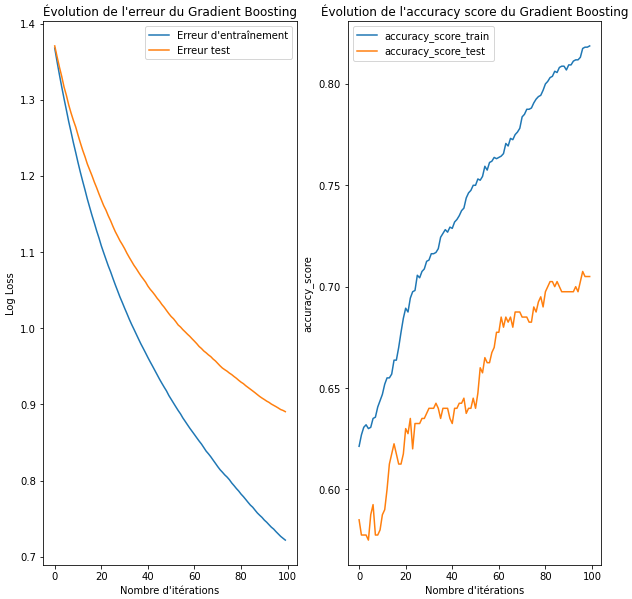
\includegraphics[width=1\linewidth]{gpt_multiclasses.png}
			\caption*{}
			
	\end{figure}\end{minipage}
	
\end{frame}

\section{Data challenge}
\begin{frame}
	\frametitle{Biosonar - Détection de clics d’Odontocètes}
	\centering
	\begin{minipage}[c]{0.6\linewidth}\centering\begin{figure}
			
			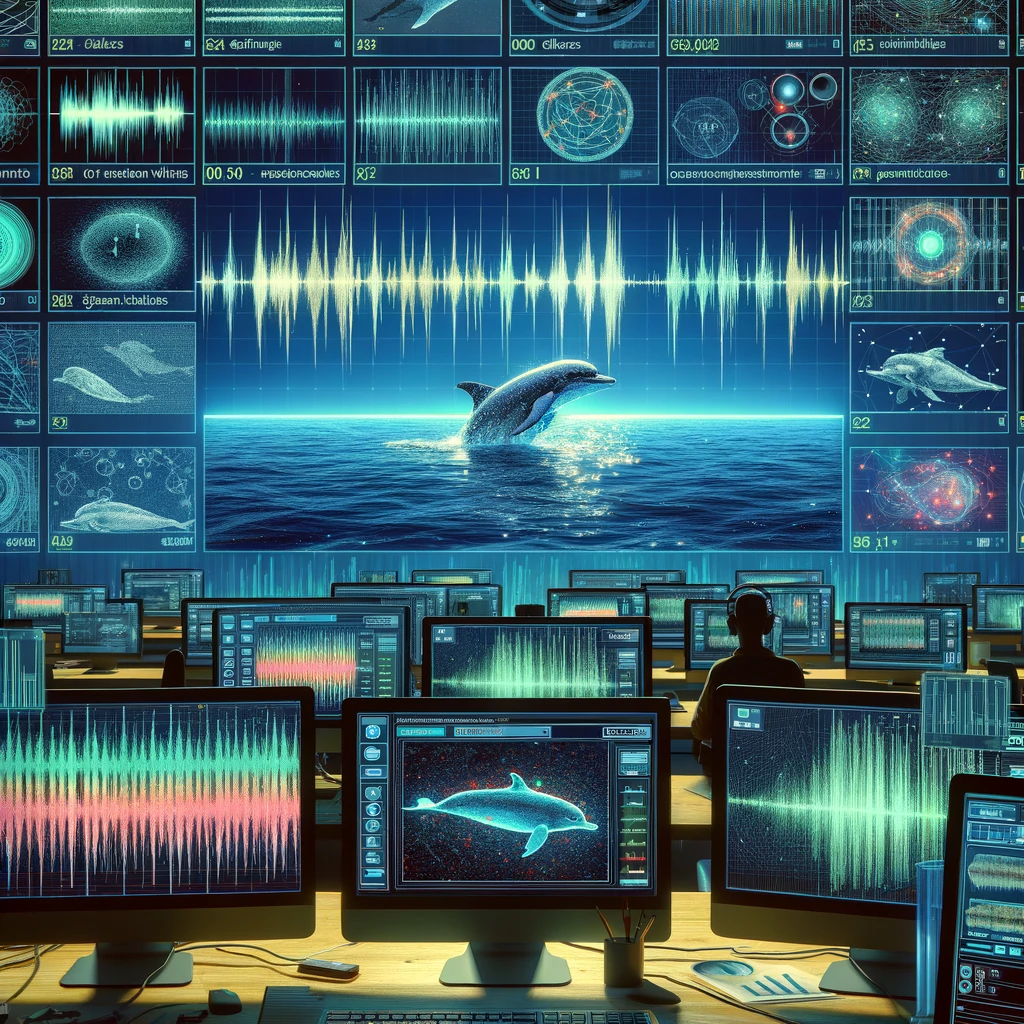
\includegraphics[width=1\linewidth]{dauphin.png}
			\caption*{}
			
	\end{figure}\end{minipage}
\end{frame}

\begin{frame}
	\frametitle{Visualisation des données et preprocessing}
	\begin{minipage}[t]{1\linewidth}
		\begin{minipage}[c]{0.51\linewidth}\centering\begin{figure}
				\centering
				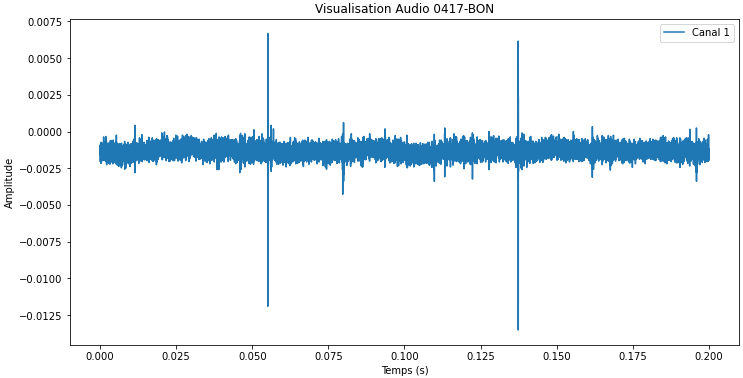
\includegraphics[width=1\linewidth]{14.png}\\[0.25cm]
				
		\end{figure}\end{minipage}\hfill 
		\begin{minipage}[c]{0.45\linewidth}\centering\begin{figure}
				\begin{center}
					\centering
					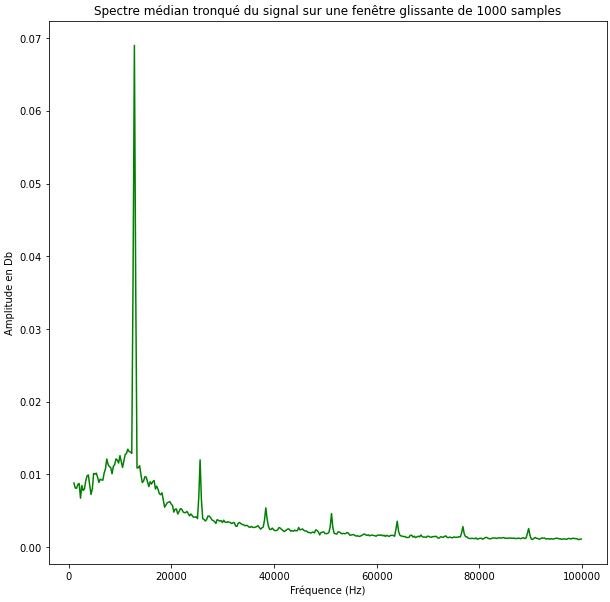
\includegraphics[width=0.8\linewidth]{13.png}
				\end{center}
		\end{figure}\end{minipage}
	\end{minipage}
\begin{center}
	\centering
	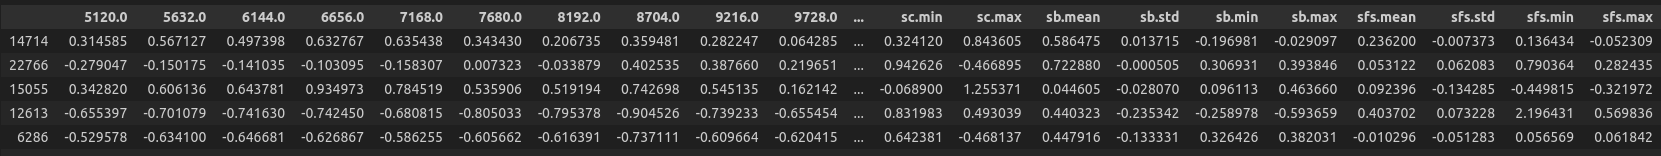
\includegraphics[width=1\linewidth]{data.png}
\end{center}	
\end{frame}

\begin{frame}
	\frametitle{Modèle de deep learning type MLP }
	\begin{minipage}[t]{1\linewidth}
		\begin{minipage}[t]{0.42\linewidth}\centering\begin{figure}
				\centering
				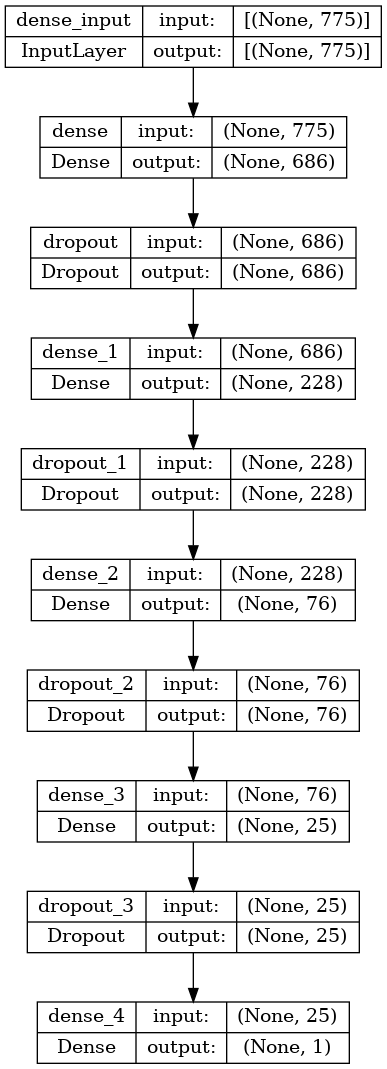
\includegraphics[width=0.5\linewidth]{model1.png}\\[0.25cm]
				
		\end{figure}\end{minipage}\hfill 
		\begin{minipage}[t]{0.53\linewidth}\centering\begin{figure}
				\begin{center}
					\centering
					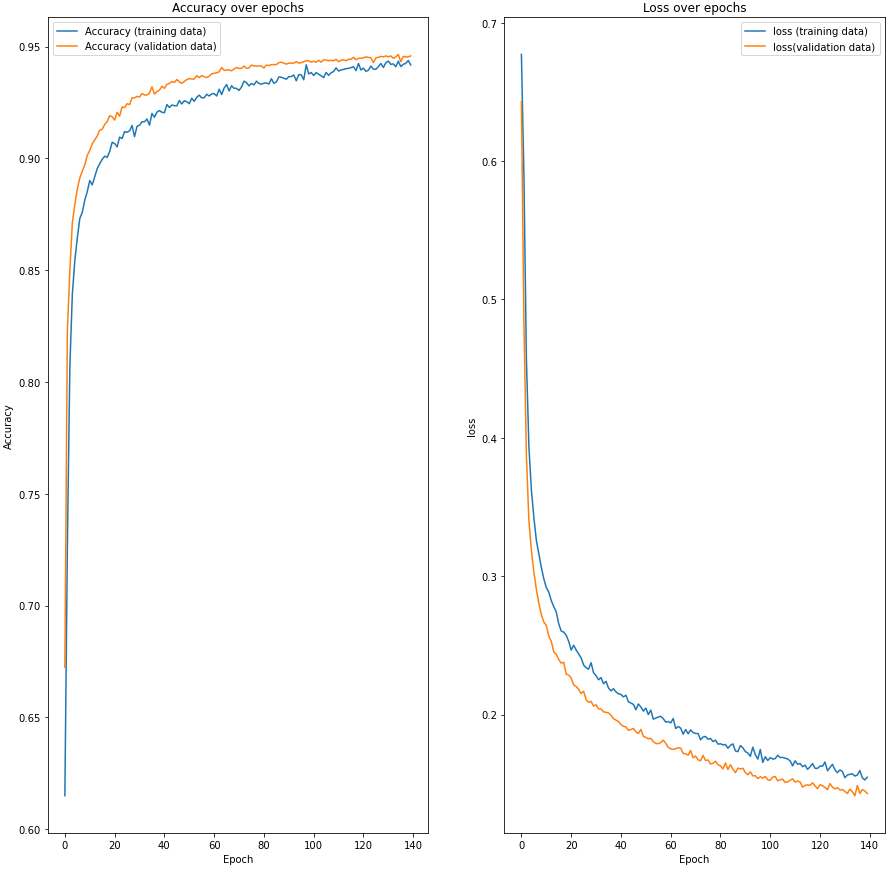
\includegraphics[width=0.7\linewidth]{15.png}
					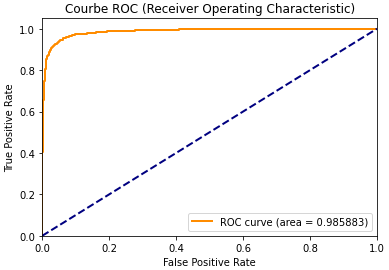
\includegraphics[width=0.7\linewidth]{16.png}
				\end{center}
				
		\end{figure}\end{minipage}
	\end{minipage}	
\end{frame}

\begin{frame}
	\frametitle{Modèle de deep learning type CNN }
	\begin{minipage}[t]{1\linewidth}
		\begin{minipage}[t]{0.42\linewidth}\centering\begin{figure}
				\centering
				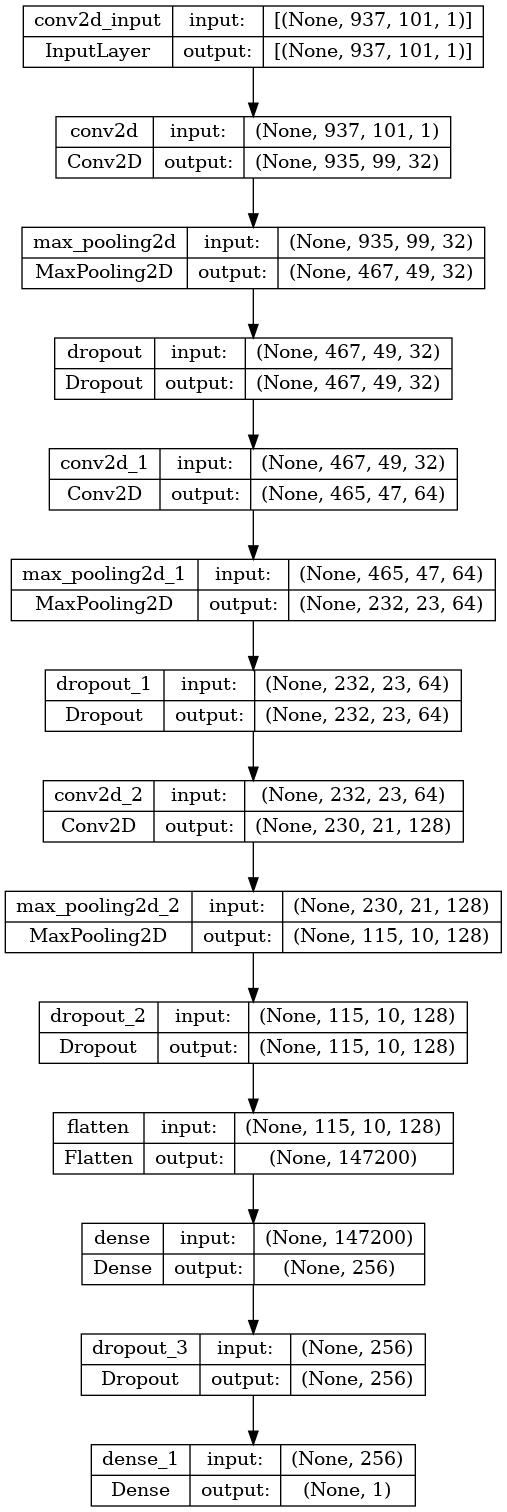
\includegraphics[width=0.5\linewidth]{model2.png}\\[0.25cm]
				
		\end{figure}\end{minipage}\hfill 
		\begin{minipage}[t]{0.55\linewidth}\centering\begin{figure}
				\begin{center}
					\centering
					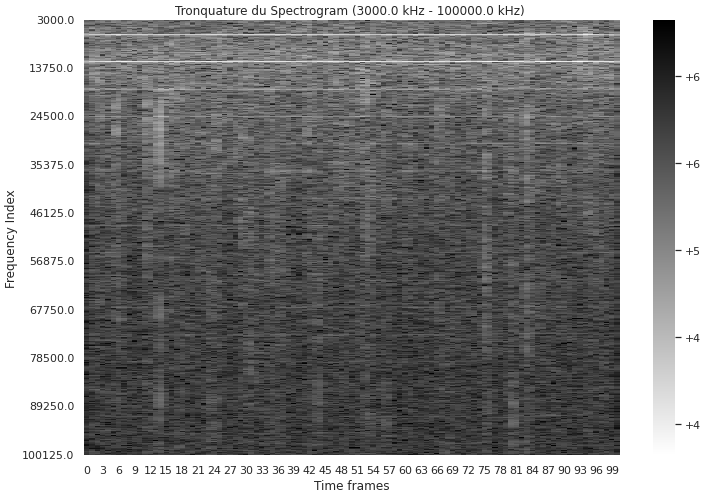
\includegraphics[width=0.8\linewidth]{19.png}\\
					
					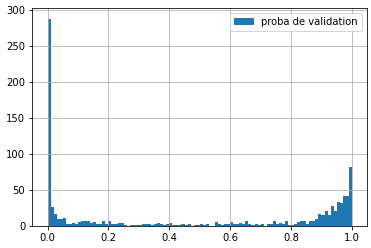
\includegraphics[width=0.8\linewidth]{val.png}
				\end{center}
				
		\end{figure}\end{minipage}
	\end{minipage}	
\end{frame}
\title{Merci pour votre écoute}
\author{}
\date{}
\begin{frame}[plain]
\maketitle\hfill\\[-3cm]
\centering	
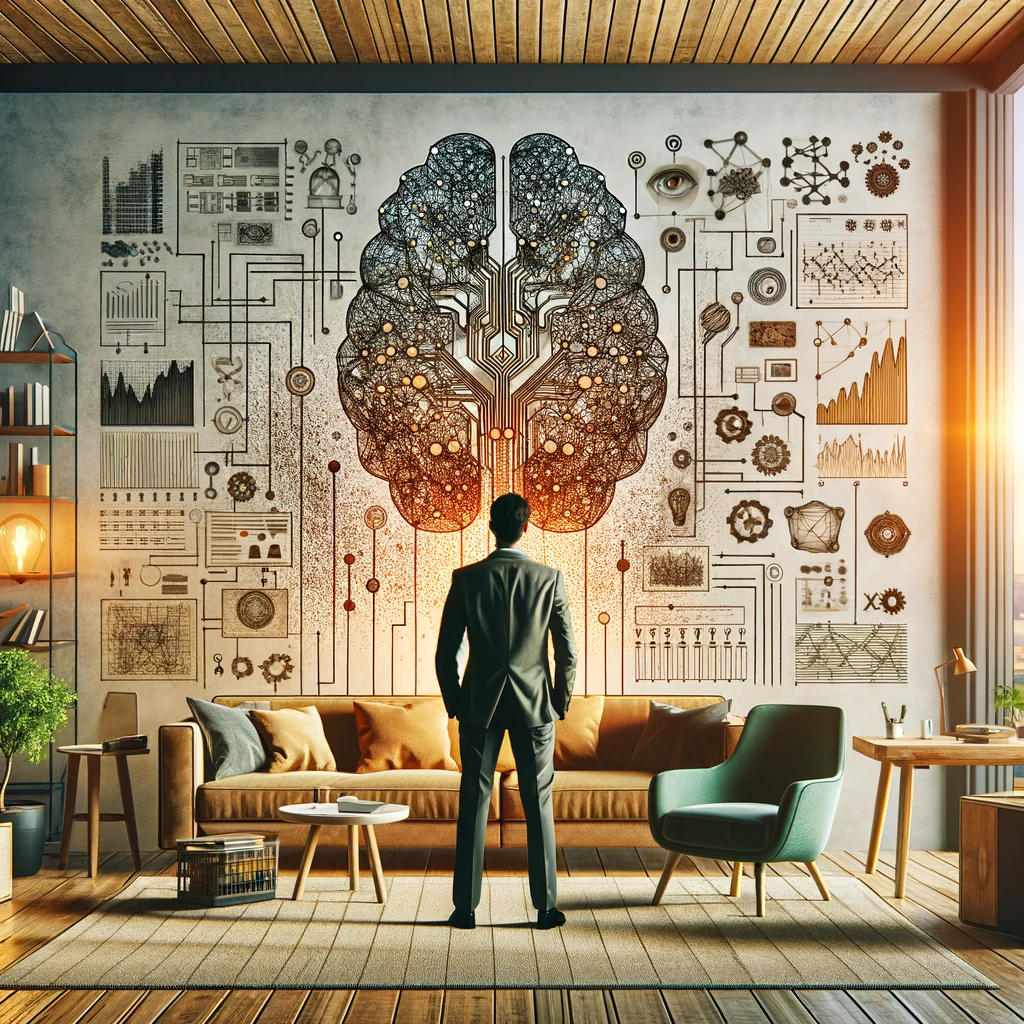
\includegraphics[width=0.6\linewidth]{end.png}
\end{frame}

\end{document}








